
%(BEGIN_QUESTION)
% Copyright 2015, Tony R. Kuphaldt, released under the Creative Commons Attribution License (v 1.0)
% This means you may do almost anything with this work of mine, so long as you give me proper credit

Denne produksjonsprosessen produserer {\it ammoniumnitrat}, en hovedbestanddel i kunstgjødsel, ved kjemisk kombinasjon av salpetersyre og ammoniakk:

$$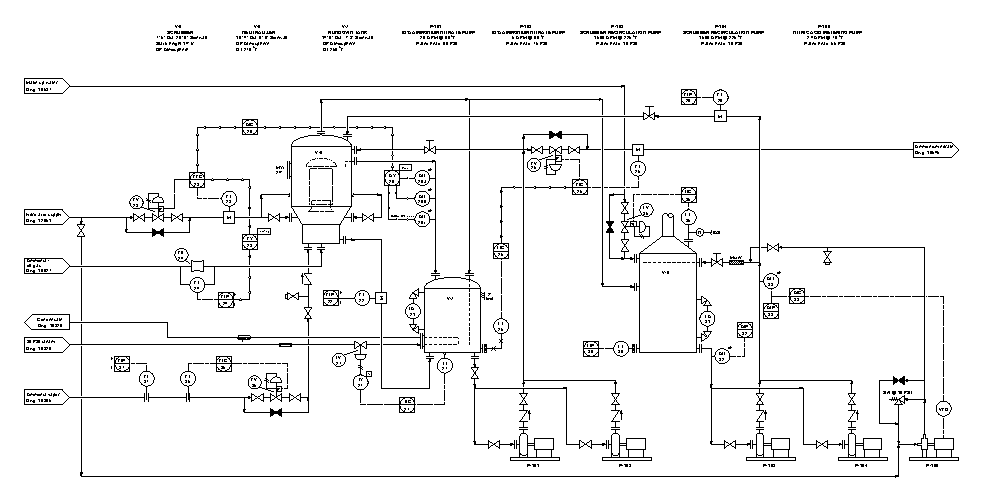
\includegraphics[width=15.5cm]{i0008rx01.eps}$$

I denne prosessen reguleres pH i væsken inne i scrubber-beholderen (V-5) ved å tilsette salpetersyre, som driver pH ned til lavere verdier, siden ammoniakkdamp som går inn i beholderen driver pH opp.

\vskip 10pt

Undersøk pH-reguleringssystemet for denne scrubber-beholderen og identifiser en av lastene i reguleringssløyfen. Etter at du har identifisert lasten, legg til en transmitter som måler denne lastvariabelen, og legg til nødvendige reguleringsfunksjoner for å implementere en {\it feedforward}-strategi for nivåreguleringen i runoff-tanken.

\underbar{file i01278}
%(END_QUESTION)





%(BEGIN_ANSWER)

\noindent
{\bf Delvis svar:}

\vskip 10pt

Kanskje den mest betydelige lasten i scrubber-beholderens pH-reguleringssløyfe er innkommende ammoniakkdampflow fra toppen av nøytraliseringsbeholderen (V-6), siden endringer i denne flowen vil endre hvor raskt ammoniakkdampen reagerer og øker pH i scrubbervannet.

%(END_ANSWER)





%(BEGIN_NOTES)

Feedforward-transmitteren for denne lasten vil naturligvis være en flowtransmitter plassert i linjen som fører ammoniakkdamp fra V-6 til V-5. Signalet fra denne transmitteren går gjennom en gain/bias-funksjon og deretter (eventuelt) gjennom en lead/lag-funksjon før det går inn i en summer-funksjon plassert mellom AIC-33 og VFD-en som driver doseringspumpen for salpetersyre (P-105). På denne måten legges det proporsjonerte feedforward-signalet til utgangen fra pH-regulator AIC-33, slik at det bestilles mer eller mindre salpetersyre inn i scrubber-beholderen før en endring rekker å måles i pH i væsken.
 
\vskip 10pt

Den nye summer-funksjonen må {\it legge til} signalet for ammoniakkdampflow til VFD-hastighetskommandoen (dvs. inngangen til summeren må være ikke-inverterende) for å få riktig retning på feedforward-virkningen: mer syre tilført for å kompensere for mer ammoniakk.


%INDEX% Control, strategies: feedforward
%INDEX% Process: ammonium nitrate production (realistic P&ID shown)

%(END_NOTES)

